% Source: inputs/original_01.pdf p.4 (printed 6-8), solution 5(1).
% Circle (x-2)^2+(y+1)^2=4; line x-y=3; A,B intersections; P=(3/2,-3/2).
\usetikzlibrary{arrows.meta,calc}
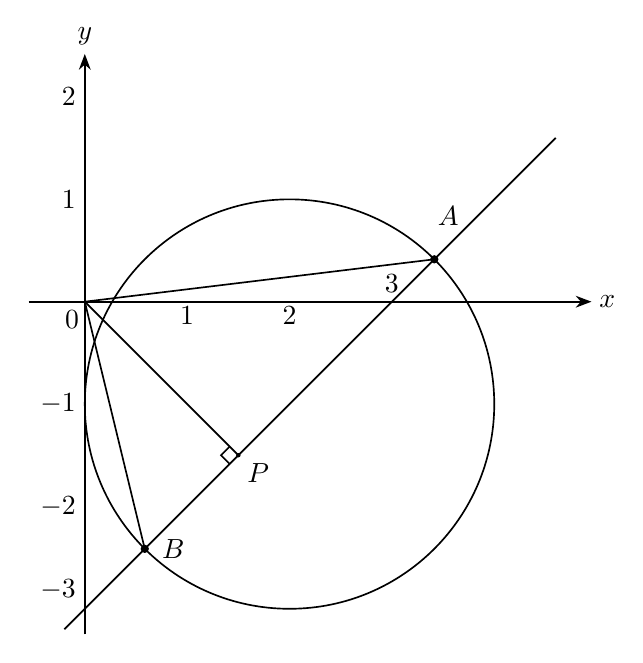
\begin{tikzpicture}[x=1.3cm,y=1.3cm,line width=.6pt,font=\normalsize,>=Stealth]
  \coordinate (O) at (0,0);
  \coordinate (C) at (2,-1);
  \coordinate (A) at (3.414214,0.414214);
  \coordinate (B) at (0.585786,-2.414214);
  \coordinate (P) at (1.5,-1.5);
  \coordinate (L1) at (-0.2,-3.2);
  \coordinate (L2) at (4.6,1.6);

  \draw[->] (-0.55,0)--(4.95,0);
  \draw[->] (0,-3.25)--(0,2.42);
  \node[anchor=west,inner sep=0pt] at (5.02,0) {$x$};
  \node[anchor=south,inner sep=0pt] at (0,2.50) {$y$};

  \draw (C) circle[radius=2];
  \draw (L1)--(L2);
  \draw (O)--(A);
  \draw (O)--(B);
  \draw (O)--(P);

  \fill (A) circle (1.5pt);
  \fill (B) circle (1.5pt);
  \fill (P) circle (0.8pt);

  \coordinate (RA1) at (1.415,-1.415);
  \coordinate (RA2) at (1.330,-1.500);
  \coordinate (RA3) at (1.415,-1.585);
  \draw (RA1)--(RA2)--(RA3);

  \node[anchor=south west,inner sep=0pt] at (3.44,0.74) {$A$};
  \node[right=5pt,inner sep=1pt] at (B) {$B$};
  \node[anchor=north west,inner sep=0pt] at (1.58,-1.57) {$P$};

  \node[anchor=north east,inner sep=0pt] at (-0.05,-0.08) {$0$};
  \node[anchor=north,inner sep=0pt] at (1,-0.04) {$1$};
  \node[anchor=north,inner sep=0pt] at (2,-0.04) {$2$};
  \node[above,inner sep=3pt] at (3,0) {$3$};
  \node[anchor=east,inner sep=0pt] at (-0.08,1) {$1$};
  \node[anchor=east,inner sep=0pt] at (-0.08,2) {$2$};
  \node[anchor=east,inner sep=0pt] at (-0.08,-1) {$-1$};
  \node[anchor=east,inner sep=0pt] at (-0.08,-2) {$-2$};
  \node[above left,inner sep=3pt] at (0,-3) {$-3$};
\end{tikzpicture}
